\section{Introduction}

This report documents the methodology and findings for Assignment 1, which explores a progression of techniques ranging from classical machine learning methods to the application of Large Language Models (LLMs). The assignment is divided into three parts:

\begin{itemize}
    \item Part 1: Regression problems.
    \item Part 2: Classical machine learning modeling using ReducedMNIST\@.
    \item Part 3: Approaches to accelerate the labeling process using advanced techniques, including LLMs.
\end{itemize}

\noindent The full simulation, plots, and numerical computations are provided in the accompanying GitHub repository: \
\href{https://github.com/EriniH/ELC4028-Neural-Networks}{ELC4028-Neural-Networks}.
\newpage

\section{Part 1: Regression Problems}
\subsection{Problem 1: Regression Analysis of Insured Persons}
\subsubsection{Problem Description}
The objective of this problem is to analyze historical data concerning the number of insured persons over a ten-year period (1987–1996) and fit an appropriate regression model. \\
The goal is to analyze the dataset for potential outliers, evaluate linear, quadratic, and cubic polynomial fits to determine the most suitable model, and ultimately predict the number of insured persons for the year 1997. 

\subsubsection{Hand Analysis}
We will first analyze the \textbf{original dataset}, then remove the outlier and refit.

\paragraph{Step 1: Transform Year for Numerical Stability} \mbox{} \\
The dataset provides the yearly count of insured persons ($y$), which is modeled against the number of years since 1987 ($x = \text{Year} - 1987$, such that $x \in \{0, 1, \dots, 9\}$). 

\begin{table}[H]
\centering
\begin{tabular}{|c|cccccccccc|}
\hline
$x$ & 0 & 1 & 2 & 3 & 4 & 5 & 6 & 7 & 8 & 9 \\
\hline
$y$ & 12400 & 10900 & 10000 & 1050 & 9500 & 8900 & 8000 & 7800 & 7600 & 7200 \\
\hline
\end{tabular}
\end{table}

\paragraph{Step 2: Fit Models (Original Data)} \mbox{} \\
We consider the following polynomial models:
\begin{align*}
\text{Linear:} \quad & y = a_0 + a_1 x \\
\text{Quadratic:} \quad & y = b_0 + b_1 x + b_2 x^2 \\
\text{Cubic:} \quad & y = c_0 + c_1 x + c_2 x^2 + c_3 x^3
\end{align*}

\subparagraph{Linear Regression Analysis} \mbox{} \\
For the original dataset with $n=10$ points, we perform a detailed linear regression analysis to fit the model $y = a_0 + a_1x$.
\textbf{Computing the Regression Coefficients:}

\begin{table}[H]
\centering
\begin{tabular}{|c|c|c|c|c|c|c|c|}
\hline
$x_i$ & $y_i$ & $(x_i - \bar{x})$ & $(y_i - \bar{y})$ & $(x_i - \bar{x})^2$ & $(y_i - \bar{y})^2$ & $(x_i - \bar{x})(y_i - \bar{y})$ \\
\hline
0 & 12400 & $-4.5$ & 4065 & 20.25 & 16524225 & $-18292.5$ \\
1 & 10900 & $-3.5$ & 2565 & 12.25 & 6579225 & $-8977.5$ \\
2 & 10000 & $-2.5$ & 1665 & 6.25 & 2772225 & $-4162.5$ \\
3 & 1050 & $-1.5$ & $-7285$ & 2.25 & 53070225 & $10927.5$ \\
4 & 9500 & $-0.5$ & 1165 & 0.25 & 1357225 & $-582.5$ \\
5 & 8900 & $0.5$ & 565 & 0.25 & 319225 & $282.5$ \\
6 & 8000 & $1.5$ & $-335$ & 2.25 & 112225 & $-502.5$ \\
7 & 7800 & $2.5$ & $-535$ & 6.25 & 286225 & $-1337.5$ \\
8 & 7600 & $3.5$ & $-735$ & 12.25 & 540225 & $-2572.5$ \\
9 & 7200 & $4.5$ & $-1135$ & 20.25 & 1288225 & $-5107.5$ \\
\hline
\multicolumn{2}{|c|}{\textbf{Sum}} & & & 82.5 & $8.29 \times 10^7$ & $-30325$ \\
\hline
\end{tabular}
\end{table}
\begin{itemize}
    \item \textbf{Mean:} $\bar{x} = \frac{0+1+2+\cdots+9}{10} = 4.5$
    \item \textbf{Mean:} $\bar{y} = \frac{\sum y_i}{10} = 8335$
\end{itemize}
Using the regression formulas:
\[
a_1 = \frac{\sum (x_i - \bar{x})(y_i - \bar{y})}{\sum (x_i - \bar{x})^2} = \frac{-30325}{82.5} \approx -367.58
\]

\[
a_0 = \bar{y} - a_1\bar{x} = 8335 - (-367.58)(4.5) = 8335 + 1654.09 \approx 9989.09
\]

Thus, the linear model for the original data is:
\[
y \approx 9989.1 - 367.6x
\]

\textbf{Steps for Computing $SSE$ and $R^2$:}
\begin{enumerate}
    \item Compute predicted values for each point using the fitted model:
    \[
    \hat{y}_i = a_0 + a_1x_i
    \]
    \item Compute residuals (prediction errors):
    \[
    e_i = y_i - \hat{y}_i
    \]
    \item Square and sum the residuals to obtain the error sum of squares:
    \[
    SSE = \sum e_i^2 = \sum (y_i - \hat{y}_i)^2
    \]
    \item Compute the total variability around the mean:
    \[
    SST = \sum (y_i - \bar{y})^2
    \]
    \item Compute the coefficient of determination:
    \[
    R^2 = 1 - \frac{SSE}{SST}
    \]
\end{enumerate}

Substituting the values for the original dataset:
\[
SSE_{\text{lin}} = \sum (y_i - \hat{y}_i)^2 \approx 7.17 \times 10^7
\]

\[
R^2_{\text{lin}} = 1 - \frac{SSE_{\text{lin}}}{SST} \approx 1 - \frac{7.17 \times 10^7}{8.29 \times 10^7} \approx 0.135
\]

\textbf{Observation:} The linear model yields a low $R^2 \approx 0.135$, indicating a poor fit. The outlier at $(x=3, y=1050)$ severely distorts the linear trend.

\subparagraph{Quadratic Model} \mbox{} \\
A quadratic model takes the form $y = b_0 + b_1 x + b_2 x^2$. 

Using the matrix method, define
\[
X = \begin{bmatrix}
1 & x_1 & x_1^2 \\
\vdots & \vdots & \vdots \\
1 & x_n & x_n^2
\end{bmatrix},
\quad
\beta = \begin{bmatrix} b_0 \\ b_1 \\ b_2 \end{bmatrix},
\quad
y = \begin{bmatrix} y_1 \\ \vdots \\ y_n \end{bmatrix}
\]
and solve the normal equations
\[
(X^T X)\beta = X^T y.
\]

For the original data ($n=10$, $x=0,\dots,9$):
\[
X^T X =
\begin{bmatrix}
10 & 45 & 285 \\
45 & 285 & 2025 \\
285 & 2025 & 15333
\end{bmatrix},
\quad
X^T y =
\begin{bmatrix}
83350 \\
344750 \\
2174650
\end{bmatrix}.
\]

Solving gives
\[
\beta =
\begin{bmatrix}
11627.73 \\
-1596.55 \\
136.55
\end{bmatrix},
\]
so the fitted quadratic model is
\[
\hat{y} = 11627.73 - 1596.55x + 136.55x^2.
\]

This model can bend around the outlier more than a line, and its fit metrics are:

\[
SSE_{\text{quad}} \approx 6.19 \times 10^7
\]

\[
R^2_{\text{quad}} \approx 1 - \frac{6.19 \times 10^7}{8.29 \times 10^7} \approx 0.253
\]

\textbf{Observation:} The quadratic model shows improvement over the linear model ($R^2$ increases from $0.135$ to $0.253$), but still provides a weak overall fit. The outlier prevents the quadratic from capturing the underlying trend across all points.

\subparagraph{Cubic Model} \mbox{} \\
A cubic model takes the form $y = c_0 + c_1 x + c_2 x^2 + c_3 x^3$.

Using the matrix method, define
\[
X = \begin{bmatrix}
1 & x_1 & x_1^2 & x_1^3 \\
\vdots & \vdots & \vdots & \vdots \\
1 & x_n & x_n^2 & x_n^3
\end{bmatrix},
\quad
\beta = \begin{bmatrix} c_0 \\ c_1 \\ c_2 \\ c_3 \end{bmatrix},
\]
and solve
\[
(X^T X)\beta = X^T y.
\]

For the original data:
\[
X^T X =
\begin{bmatrix}
10 & 45 & 285 & 2025 \\
45 & 285 & 2025 & 15333 \\
285 & 2025 & 15333 & 120825 \\
2025 & 15333 & 120825 & 978405
\end{bmatrix},
\quad
X^T y =
\begin{bmatrix}
83350 \\
344750 \\
2174650 \\
15383150
\end{bmatrix}.
\]

Solving gives
\[
\beta =
\begin{bmatrix}
13113.15 \\
-4313.93 \\
932.31 \\
-58.95
\end{bmatrix},
\]
so the fitted cubic model is
\[
\hat{y} = 13113.15 - 4313.93x + 932.31x^2 - 58.95x^3.
\]

With 4 parameters for 10 data points, the cubic model has more flexibility to bend around the outlier. Its fit metrics are:

\[
SSE_{\text{cubic}} \approx 5.11 \times 10^7
\]

\[
R^2_{\text{cubic}} \approx 1 - \frac{5.11 \times 10^7}{8.29 \times 10^7} \approx 0.383
\]

\textbf{Observation:} The cubic model exhibits the highest $R^2 \approx 0.383$, but this improvement is still largely driven by the model's increased flexibility to fit the extreme outlier rather than capturing a genuine cubic underlying trend.

\subparagraph{Conclusion for Original Data} \mbox{} \\
Although the cubic model has the highest $R^2$ value among the three models fitted to the original data, the overall poor performance across all models (even the best $R^2 \approx 0.383$ explains only about 38\% of variance) demonstrates the severe impact of the outlier. The outlier at $(x=3, y=1050)$ fundamentally distorts the regression analysis, and no simple polynomial model can adequately fit both this extreme point and the general declining trend in the remaining data. This observation motivates the need for outlier detection and removal before proceeding with final model selection.

\paragraph{Step 3: Remove Outlier} \mbox{} \\
Removing the obvious outlier $(x=3, y=1050)$ leaves $n=9$ valid points.

\paragraph{Step 4: Fit Models Without Outlier} \mbox{} \\
\subparagraph{Linear Regression Analysis} \mbox{} \\
For the remaining $n = 9$ data points, the $x$ values are $\{0, 1, 2, 4, 5, 6, 7, 8, 9\}$. The detailed computations are shown below:

\begin{table}[H]
\centering
\begin{tabular}{|c|c|c|c|c|c|c|}
\hline
$x_i$ & $y_i$ & $(x_i - \bar{x})$ & $(y_i - \bar{y})$ & $(x_i - \bar{x})^2$ & $(y_i - \bar{y})^2$ & $(x_i - \bar{x})(y_i - \bar{y})$ \\
\hline
0 & 12400 & $-4.667$ & 3255.556 & 21.778 & 10598641.98 & $-15192.59$ \\
1 & 10900 & $-3.667$ & 1755.556 & 13.444 & 3082716.05 & $-6437.04$ \\
2 & 10000 & $-2.667$ & 855.556 & 7.111 & 731975.31 & $-2281.48$ \\
4 & 9500 & $-0.667$ & 355.556 & 0.444 & 126419.75 & $-237.04$ \\
5 & 8900 & $0.333$ & $-244.444$ & 0.111 & 59753.09 & $-81.48$ \\
6 & 8000 & $1.333$ & $-1144.444$ & 1.778 & 1309753.09 & $-1525.93$ \\
7 & 7800 & $2.333$ & $-1344.444$ & 5.444 & 1807530.86 & $-3137.04$ \\
8 & 7600 & $3.333$ & $-1544.444$ & 11.111 & 2385308.64 & $-5148.15$ \\
9 & 7200 & $4.333$ & $-1944.444$ & 18.778 & 3780864.20 & $-8425.93$ \\
\hline
\multicolumn{2}{|c|}{\textbf{Sum}} & & & 80.000 & $2.39 \times 10^7$ & $-42466.67$ \\
\hline
\end{tabular}
\end{table}
\begin{itemize}
    \item \textbf{Mean:} $\bar{x} = \frac{0+1+2+4+\cdots+9}{9} = 4.667$
    \item \textbf{Mean:} $\bar{y} = \frac{\sum y_i}{9} = 9144.44$
\end{itemize}

Using the regression formulas:
\[
a_1 = \frac{\sum (x_i - \bar{x})(y_i - \bar{y})}{\sum (x_i - \bar{x})^2} = \frac{-42466.67}{80} \approx -530.83
\]

\[
a_0 = \bar{y} - a_1\bar{x} = 9144.44 - (-530.83)(4.667) = 9144.44 + 2477.23 \approx 11621.67
\]

Thus, the best-fit linear equation is:
\[
    y \approx 11621.67 - 530.83x
\]

Substituting the cleaned-data values into the previously defined $SSE$ and $R^2$ equations:
\begin{align*}
    SSE_{\text{lin}} &= \sum (y_i - \hat{y}_i)^2 \approx 1.34 \times 10^6 \\
    R^2_{\text{lin}} &= 1 - \frac{SSE_{\text{lin}}}{SST} \approx 1 - \frac{1.34 \times 10^6}{2.39 \times 10^7} \approx 0.944
\end{align*}

The linear model already provides an excellent fit with $R^2 \approx 0.944$.

\subparagraph{Quadratic Model} \mbox{} \\
A quadratic model takes the form $y = b_0 + b_1 x + b_2 x^2$.

Using the matrix method defined previously, for the cleaned data:
\[
X^T X =
\begin{bmatrix}
9 & 42 & 276 \\
42 & 276 & 1998 \\
276 & 1998 & 15252
\end{bmatrix},
\quad
X^T y =
\begin{bmatrix}
82300 \\
341600 \\
2165200
\end{bmatrix}.
\]

Solving gives
\[
\beta =
\begin{bmatrix}
12024.17 \\
-863.13 \\
37.44
\end{bmatrix},
\]
so the fitted quadratic model is
\[
\hat{y} = 12024.17 - 863.13x + 37.44x^2.
\]

Its fit metrics are:
\[
SSE_{\text{quad}} \approx 6.57 \times 10^5
\]
\[
R^2_{\text{quad}} \approx 1 - \frac{6.57 \times 10^5}{2.39 \times 10^7} \approx 0.972
\]

\textbf{Observation:} The quadratic model improves the fit over linear ($R^2$ increases from $0.944$ to $0.972$), but adds one extra parameter.

\subparagraph{Cubic Model} \mbox{} \\
A cubic model takes the form $y = c_0 + c_1 x + c_2 x^2 + c_3 x^3$.

Using the matrix method defined previously, for the cleaned data:

For the cleaned data:
\[
X^T X =
\begin{bmatrix}
9 & 42 & 276 & 1998 \\
42 & 276 & 1998 & 15252 \\
276 & 1998 & 15252 & 120582 \\
1998 & 15252 & 120582 & 977676
\end{bmatrix},
\quad
X^T y =
\begin{bmatrix}
82300 \\
341600 \\
2165200 \\
15354800
\end{bmatrix}.
\]

Solving gives
\[
\beta =
\begin{bmatrix}
12204.42 \\
-1221.74 \\
140.17 \\
-7.46
\end{bmatrix},
\]
so the fitted cubic model is
\[
\hat{y} = 12204.42 - 1221.74x + 140.17x^2 - 7.46x^3.
\]

Its fit metrics are:
\[
SSE_{\text{cubic}} \approx 5.09 \times 10^5
\]
\[
R^2_{\text{cubic}} \approx 1 - \frac{5.09 \times 10^5}{2.39 \times 10^7} \approx 0.979
\]

\textbf{Observation:} The cubic model gives the highest $R^2$, but the improvement from quadratic ($0.972 \to 0.979$) is modest relative to the extra complexity.

\subparagraph{Conclusion for Cleaned Data} \mbox{} \\
All three models fit the cleaned dataset well. However, following the same model-selection principle used in Step 2 (favor simpler models unless improvement is substantial), the linear model remains the preferred choice for interpretation and forecasting. Although quadratic and cubic models increase $R^2$, the linear trend already captures the dominant behavior after outlier removal and avoids unnecessary model complexity.

\paragraph{Step 5: Predict for 1997} \mbox{} \\
The year 1997 corresponds to $x=10$ (since $x=\text{Year}-1987$).
Using the linear model $y = 11621.67 - 530.83x$:
\[
y_{1997} = 11621.67 - 530.83(10) = 11621.67 - 5308.30 = 6313.37
\]

Thus, the predicted number of insured persons in 1997 is approximately $\boxed{6313}$.

\subsubsection{Simulation Analysis}

\paragraph{(a) Model Fitting and $R^2$ Comparison} \mbox{} \\
A scatterplot of the original data shows a generally decreasing trend with a sharp drop at $x=3$. We fit linear, quadratic, and cubic models and compute $R^2$:

\begin{figure}[H]
    \centering
    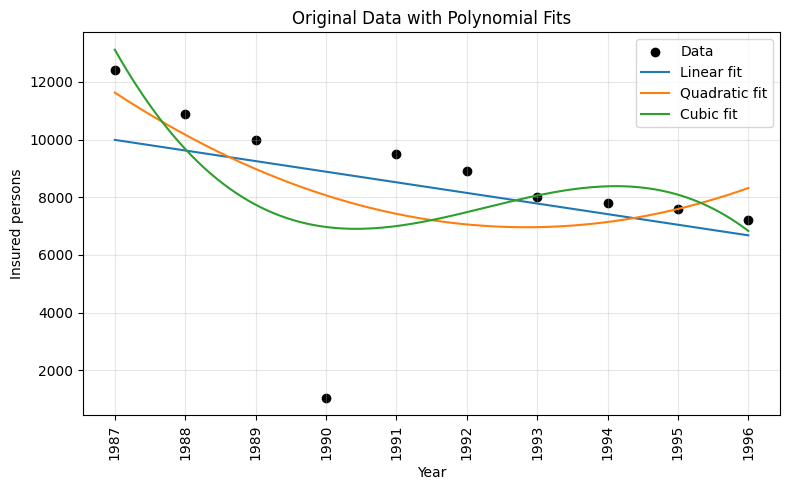
\includegraphics[width=0.6\textwidth]{figures/Original Data with Polynomial Fits.png}
    \caption{Scatterplot of insured persons vs. years since 1987 with polynomial fits (original data)}
    \label{fig:scatter}
\end{figure}

\begin{figure}[H]
    \centering
    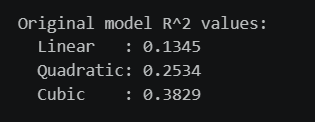
\includegraphics[height=0.15\textwidth]{figures/Original R-Squared.png}
    \caption{R-squared values for the original data}
    \label{fig:originalr2}
\end{figure}

\textbf{Observation:} All models yield relatively low $R^2$ values. Even the cubic model explains less than $40\%$ of the variance, indicating a poor overall fit due to the outlier.

\textbf{Conclusion:} Although the cubic model has the highest $R^2$, the improvement is artificially limited and does not adequately capture the generalized data behavior.

\paragraph{(b) Outlier Removal and Re-fitting} \mbox{} \\
From the initial scatterplot, the point $(x=3, y=1050)$ is clearly outside the general trend and rightfully treated as an outlier. After removing this point, the data demonstrates a strong linear decreasing pattern.

\begin{figure}[H]
    \centering
    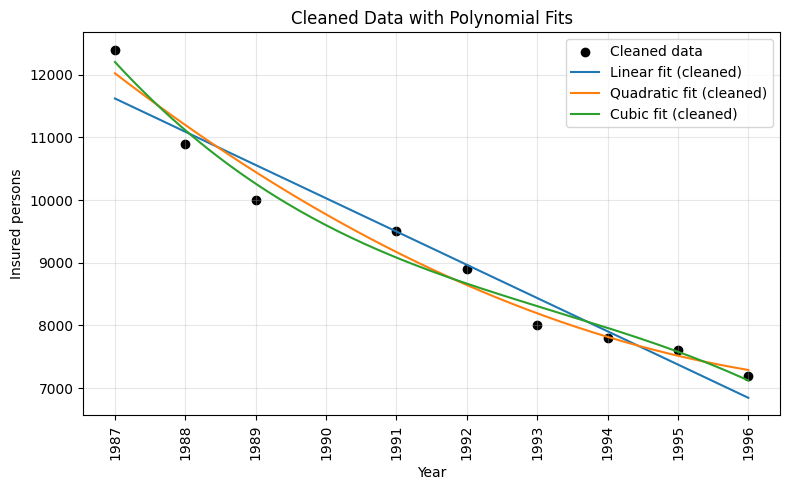
\includegraphics[width=0.6\textwidth]{figures/Cleaned Data with Polynomial Fits.png}
    \caption{Scatterplot of insured persons vs. years since 1987 with polynomial fits (cleaned data)}
    \label{fig:scatter2}
\end{figure}

Recomputing the models yields the following metrics:

\begin{figure}[H]
    \centering
    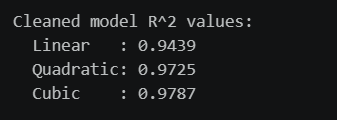
\includegraphics[height=0.15\textwidth]{figures/Cleaned R-Squared.png}
    \caption{R-squared values for cleaned data}
    \label{fig:cleanr2}
\end{figure}

\textbf{Conclusion:} The linear model already provides an excellent fit. Higher-order models offer only marginal mathematical improvement and introduce unnecessary complexity.
\[
\boxed{\text{Best model: Linear}}
\]

\paragraph{(c) Graphical Representation} \mbox{} \\
The scatterplot for the cleaned data is plotted along with the best-fit linear function:
\[
y \approx 11621.67 - 530.83x
\]
The fitted line closely follows the data trend after outlier removal, visually validating our model choice.

\paragraph{(d) Prediction for 1997} \mbox{} \\
For the year 1997 ($x = 10$):

\begin{figure}[H]
    \centering
    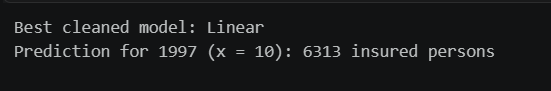
\includegraphics[width=0.6\textwidth]{figures/Prediction.png}
    \caption{Best cleaned model providing a forecast for 1997}
    \label{fig:p1_prediction_1997}
\end{figure}

Using the best-fit linear model:
\[
y = 11621.67 - 530.83(10) = 6313.37
\]
\[
\boxed{y_{1997} \approx 6313}
\]

\paragraph{Final Interpretation} \mbox{} \\
The presence of the single outlier significantly degraded the initial model performance. After removing it, the dataset is very well-described by a simpler linear model, which ultimately provides a more reliable and robust prediction for future values.
\newpage
\subsection{Problem 2: Regression Analysis of Heating Oil Usage}
\subsubsection{Problem Description}
Develop a model for estimating heating oil used for a single-family home in January based on average temperature and amount of insulation in inches.

\begin{table}[h!]
\centering
\begin{tabular}{c|c|c}
Oil & Temp F & Insulation \\
\hline
270 & 40 & 4 \\
362 & 27 & 4 \\
162 & 40 & 10 \\
45 & 73 & 6 \\ 
91 & 65 & 7 \\
233 & 65 & 40 \\
372 & 10 & 6 \\
305 & 9 & 10 \\
234 & 24 & 10 \\
122 & 65 & 4 \\
25 & 66 & 10 \\
210 & 41 & 6 \\
450 & 22 & 4 \\
325 & 40 & 4 \\
52 & 60 & 10 \\
\hline
\end{tabular}
\end{table}
\subsubsection{Simulation Analysis}
\textbf{(a) Model Fitting and $R^2$ Comparison}
We fit linear and quadratic models and compute $R^2$:

\begin{figure}[H]
    \centering
    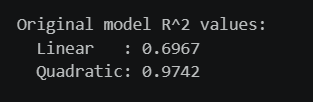
\includegraphics[height=0.15\textwidth]{figures/P2 orig.png}
    \caption{R-squared values for the original data}
    \label{fig:originalr2p2}
\end{figure}

\textbf{Observation:}  
The quadratic model $R^2$ value is higher than the linear model. The quadratic model fits the data better, but this judgement is affected by the outliers, so it is unreliable.

\textbf{Conclusion:}  
Although the quadratic model has the highest $R^2$, we can't tell if it adequately capture the data behavior.


\vspace{.4cm}
\textbf{(b) Outlier Removal and Re-fitting}
the point $(Insulation=400)$ is clearly outside the general trend and is treated as an outlier.

Recomputing the models:

\begin{figure}[H]
    \centering
    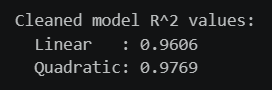
\includegraphics[height=0.15\textwidth]{figures/P2 clean.png}
    \caption{R-squared values for cleaned data}
    \label{fig:cleanr2p2}
\end{figure}

\textbf{Conclusion:}  
The linear model already provides an excellent fit. Higher-order models offer only marginal improvement and introduce unnecessary complexity.

\[
\boxed{\text{Best model: Linear}}
\]

\vspace{.4cm}
\textbf{(c) Prediction for temperature $15^\circ$F and insulation 5 inches}

For temperature $15^\circ$F and insulation 5 inches:
\begin{figure}[H]
    \centering
    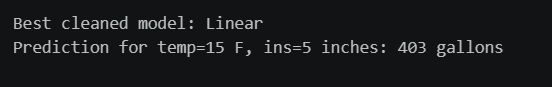
\includegraphics[height=0.15\textwidth]{figures/P2 pred.png}
    \caption{Best cleaned model and prediction for temperature $15^\circ$F with insulation 5 inches}
    \label{fig:p2_prediction_oil}
\end{figure}

\textbf{Final Interpretation:}  
The presence of the outlier significantly degrades model performance. After removing it, the data is well-described by a linear model, which provides a reliable prediction for future values.
\newpage

\section{Part 2: ReducedMNIST Classification}
Part 2 uses ReducedMNIST, a reduced version of the MNIST dataset, with the following assignment-compliant split:

\begin{itemize}
    \item Original MNIST training set: 60,000 images total.
    \item Original MNIST test set: 10,000 images total.
    \item The script \texttt{part2\_reduced\_mnist.py} downloads MNIST and creates a reduced version of the dataset, called ReducedMNIST, with the following split:
        \begin{itemize}
            \item ReducedMNIST training set: 1000 images for each digit (10000 total).
            \item ReducedMNIST test set: 200 images for each digit (2000 total).
        \end{itemize}
\end{itemize}

\subsection{Feature Extraction}

Three feature extraction methods were used:

\begin{itemize}
    \item \textbf{DCT}: a $15 \times 15$ low-frequency block, giving 225 features.
    \item \textbf{PCA}: enough principal components to preserve at least 95\% of the total variance.
    \item \textbf{HOG}: histogram-of-oriented-gradients features extracted from each image.
\end{itemize}

\subsection{Classifiers}

Two classifier families were evaluated:

\begin{itemize}
    \item \textbf{K-means clustering per class} with $K = 1, 4, 16, 32$.
    \item \textbf{SVM} with a linear kernel and a nonlinear kernel.
\end{itemize}

For the nonlinear SVM result, the kernel used was \textbf{RBF} with \texttt{gamma = scale}.

\subsection{Results Summary}

Table~\ref{tab:part2_results} summarizes the final Part 2 results. Processing time is the total of feature extraction, training, and testing.

\begin{table}[H]
\centering
\caption{Part 2 comparison of features and classifiers}
\label{tab:part2_results}
\resizebox{\textwidth}{!}{
\begin{tabular}{llcccccc}
\toprule
\multicolumn{2}{c}{\textbf{}} & \multicolumn{2}{c}{\textbf{DCT}} & \multicolumn{2}{c}{\textbf{PCA}} & \multicolumn{2}{c}{\textbf{HOG}} \\
\cmidrule(lr){3-4} \cmidrule(lr){5-6} \cmidrule(lr){7-8}
\textbf{Classifier} & \textbf{Setting} & \textbf{Accuracy} & \textbf{Processing Time} & \textbf{Accuracy} & \textbf{Processing Time} & \textbf{Accuracy} & \textbf{Processing Time} \\
\midrule
K-means Clustering & 1  & 78.10\% & 1.8831 s & 85.20\% & 0.8123 s & 89.50\% & 5.4810 s \\
K-means Clustering & 4  & 84.40\% & 1.0484 s & 82.60\% & 1.1766 s & 92.00\% & 7.3776 s \\
K-means Clustering & 16 & 88.75\% & 2.2338 s & 85.70\% & 2.1196 s & 94.35\% & 13.5238 s \\
K-means Clustering & 32 & 89.65\% & 3.8399 s & 85.60\% & 3.5880 s & 93.95\% & 21.7835 s \\
SVM & Linear      & 90.25\% & 2.3988 s & 90.65\% & 3.1937 s & 97.45\% & 11.2708 s \\
SVM & Nonlinear*  & 95.55\% & 4.2029 s & 95.15\% & 5.5291 s & 97.15\% & 24.9506 s \\
\bottomrule
\end{tabular}
}
\end{table}

\noindent * Nonlinear kernel = RBF, \texttt{gamma = scale}.

\subsection{Best Results and Confusion Matrices}

The best K-means result was \textbf{K-means with $K=16$ using HOG}, with an accuracy of \textbf{94.35\%}. The best SVM result was \textbf{linear SVM using HOG}, with an accuracy of \textbf{97.45\%}. As required by the assignment, only the best result from each classifier family is shown as a confusion matrix.

\begin{figure}[H]
\centering
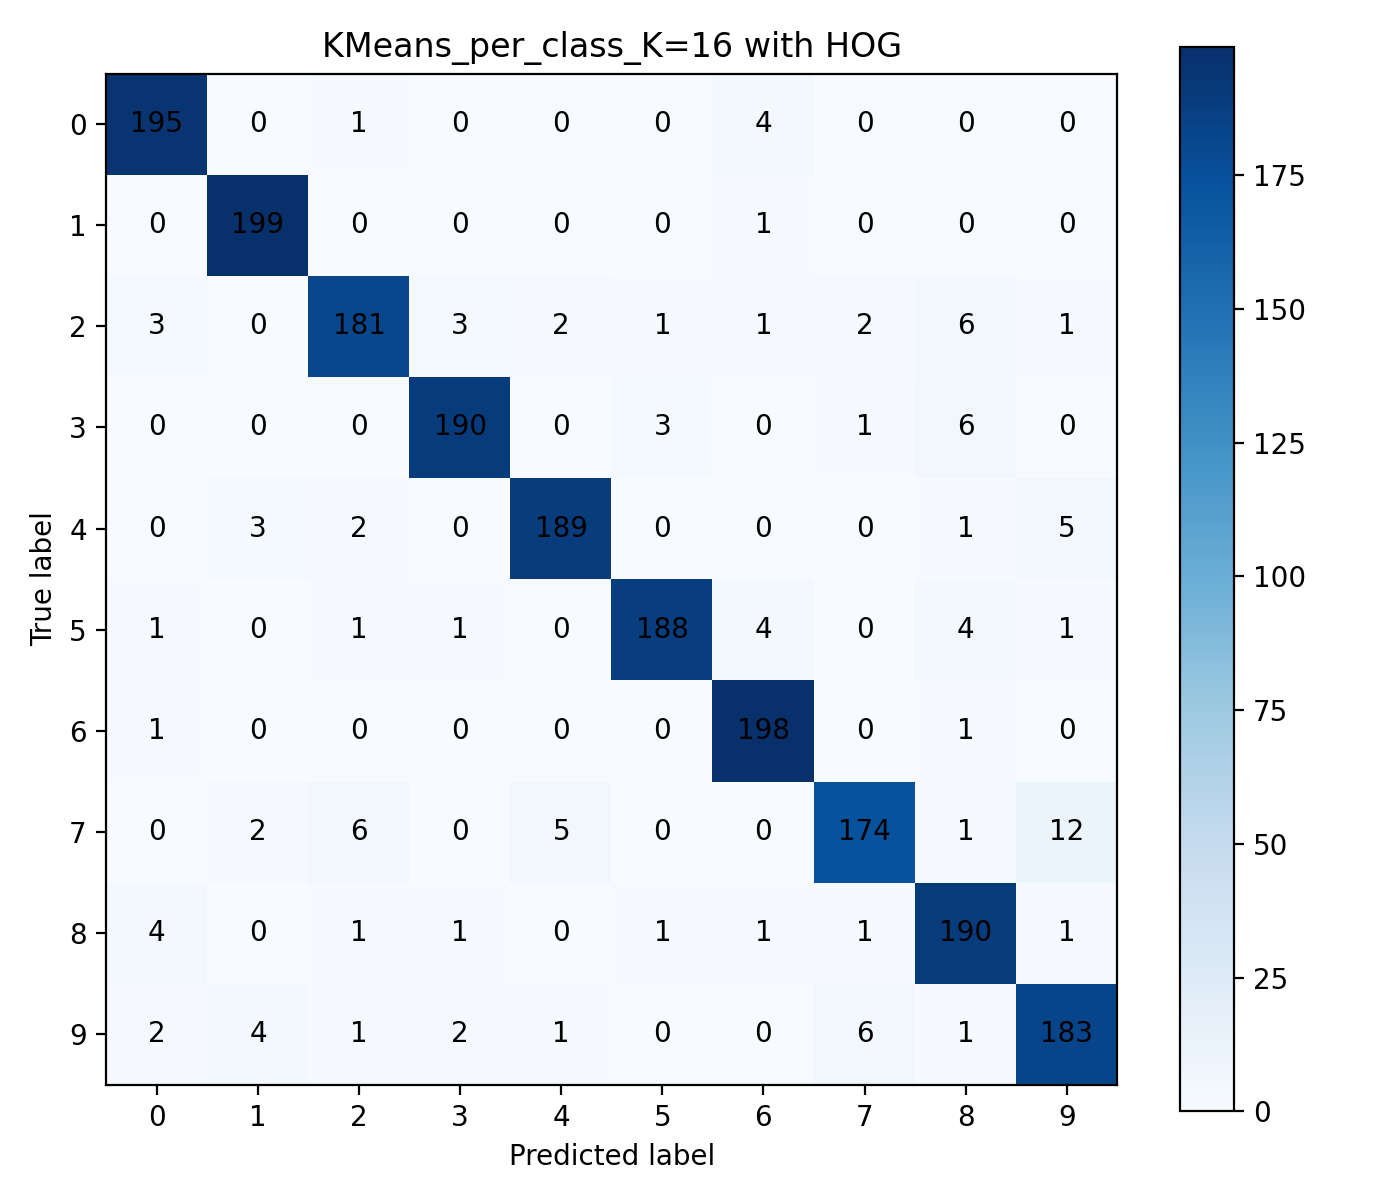
\includegraphics[width=0.68\textwidth]{figures/KMeans_per_class_K=16_HOG_confusion.png}
\caption{Confusion matrix for the best K-means result: K-means ($K=16$) with HOG features.}
\end{figure}

\begin{figure}[H]
\centering
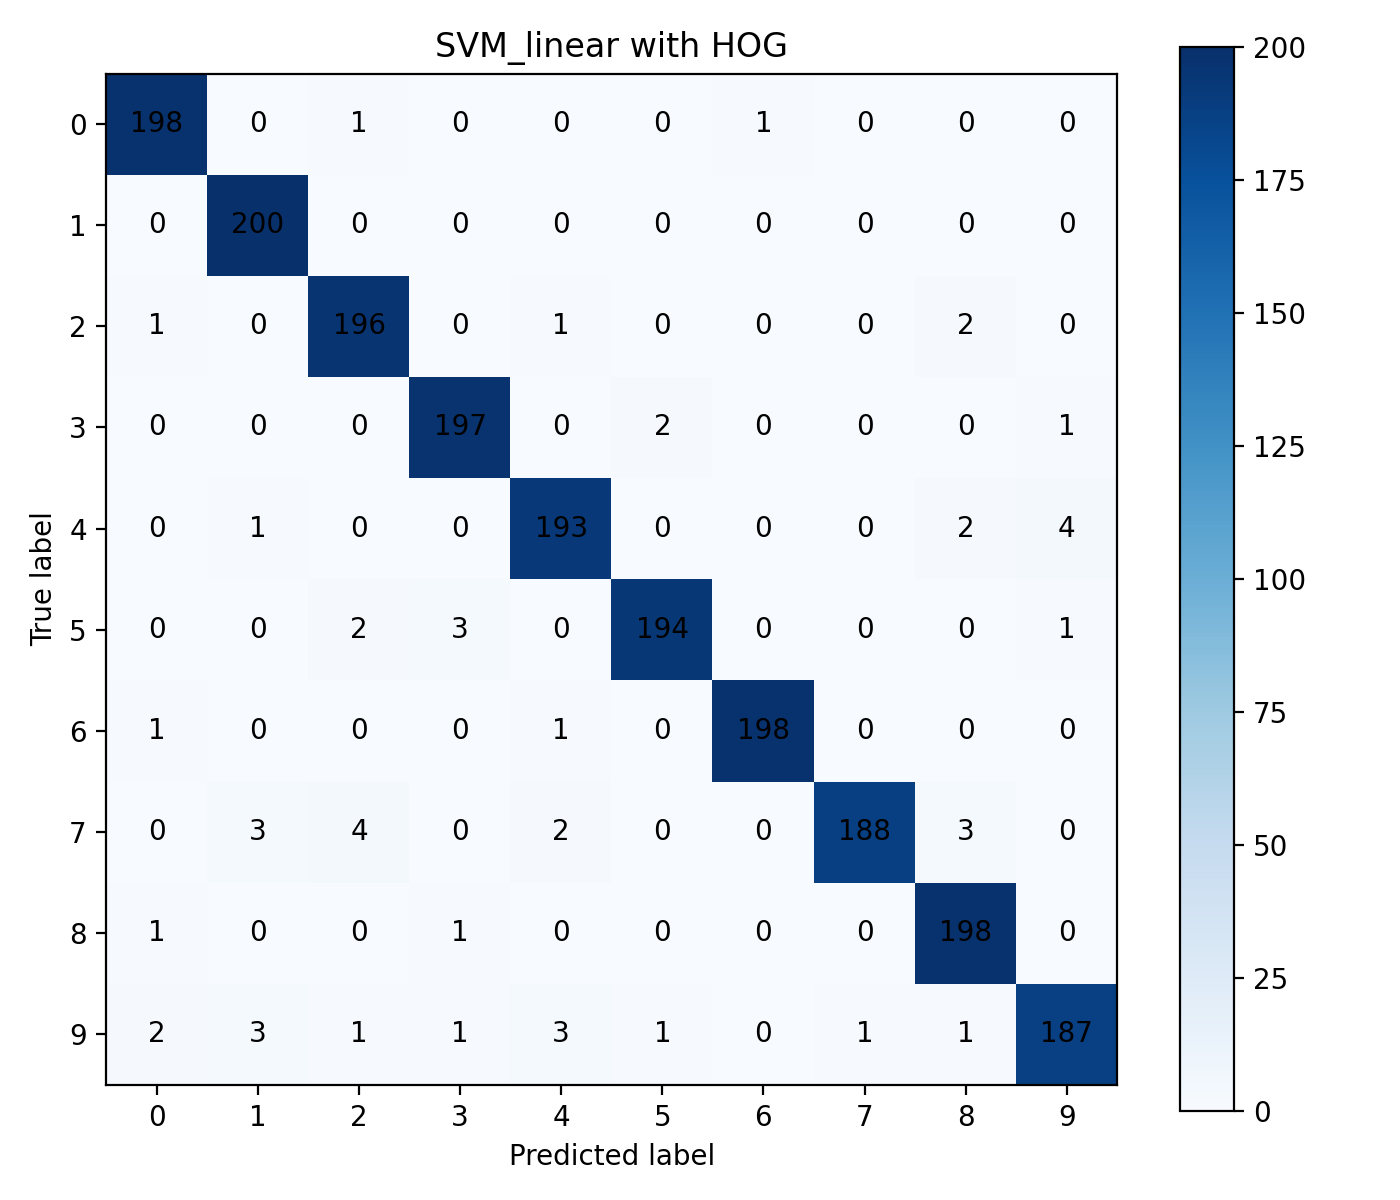
\includegraphics[width=0.68\textwidth]{figures/SVM_linear_HOG_confusion.png}
\caption{Confusion matrix for the best SVM result: linear SVM with HOG features.}
\end{figure}

\subsection{Observations}

The results show that HOG features produced the strongest classification accuracy across both classifier families. The best overall result was obtained by \textbf{linear SVM with HOG}, reaching \textbf{97.45\%}. The best K-means result, \textbf{K=16 with HOG}, reached \textbf{94.35\%}, so the best SVM result was \textbf{3.10 percentage points} higher.

For DCT and PCA, the nonlinear SVM result was slightly better than the linear SVM result. For HOG, however, the linear SVM result was the strongest overall result in the full comparison table. In terms of speed, the fastest overall experiment was \textbf{K-means with $K=1$ using PCA}, with a total processing time of \textbf{0.8123 s}, but with lower accuracy than the best SVM and HOG-based results.

\subsection{Part 2 Conclusion}

Based on the current experiments, \textbf{HOG features combined with linear SVM} gave the best overall performance for the ReducedMNIST classification task. HOG consistently captured the digit structure better than DCT and PCA in the final results, while linear SVM achieved the highest measured test accuracy with a reasonable processing time.
\newpage

\section{Part 3: Ways to Fasten the Labelling Process}
This part is organized into three separate pipelines. Each pipeline will have its own method description, block diagram with exact settings and observed values, manual-effort estimate, and final accuracy results. The pipelines are designed to explore different strategies for reducing manual labeling effort while maintaining high accuracy.
\subsection{Pipeline 1: K-means Bootstrapping + Human-in-the-Loop SVM}
The goal is to reduce direct one-by-one manual labeling by first labeling coherent clusters, then correcting only uncertain boundary samples.
\subsubsection{Problem Statement and Setup}
\begin{itemize}
    \item Dataset: 10,000 grayscale digit images (Indian digits), resolution $28 \times 28$.
    \item Feature representation: \textbf{HOG} with 1296 dimensions.
    \item Clustering stage: \textbf{K-means with fixed $K=50$} (5 clusters per class on average).
    \item Human cluster review: 8 sampled images per cluster, then assign one label or mark cluster as mixed.
    \item Refinement stage: weighted SVM + least-confidence boundary labeling in batches.
\end{itemize}

\subsubsection{Block Diagram (Exact Steps and Values)}
\begin{figure}[H]
\centering
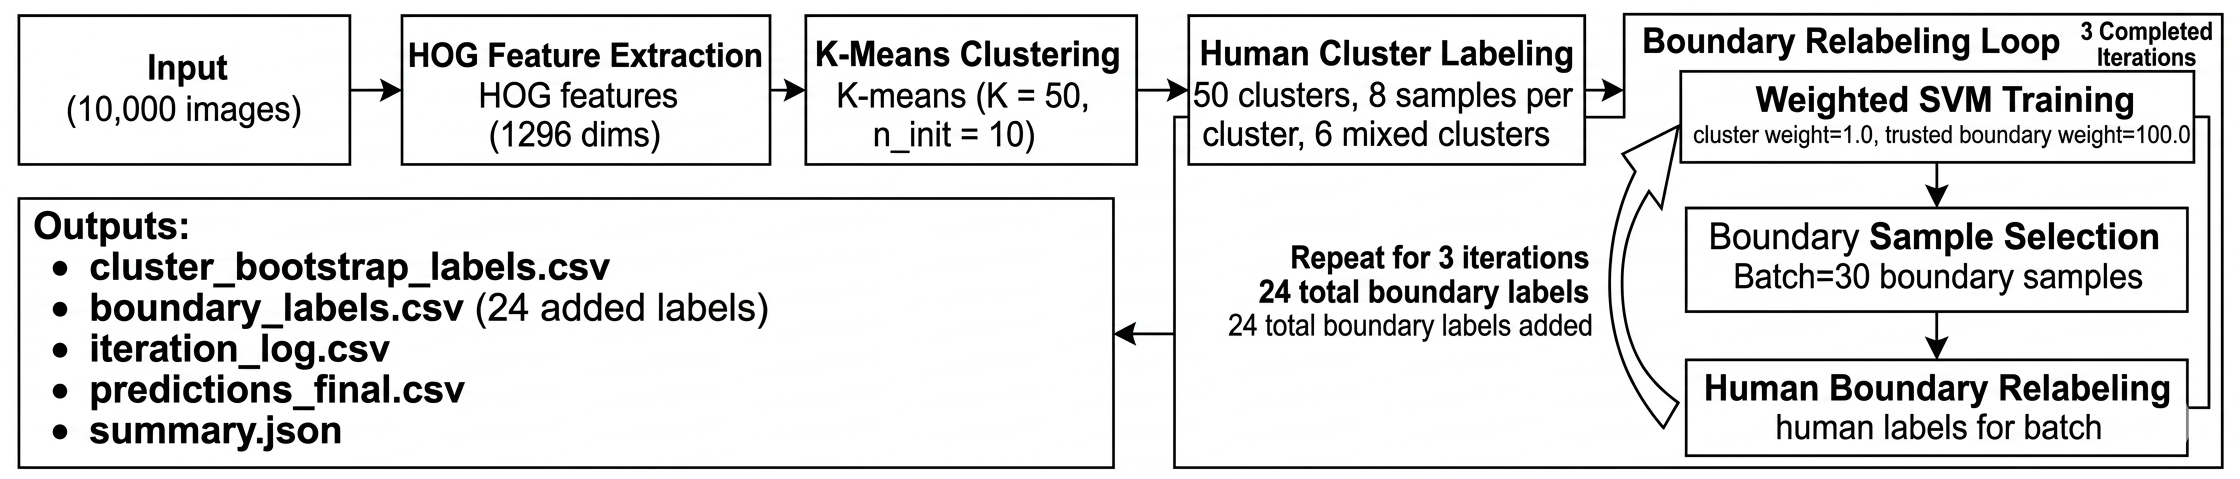
\includegraphics[width=0.96\textwidth]{figures/pipeline1_blockdiagram.png}
\caption{Pipeline 1 block diagram with exact run settings and observed values.}
\label{fig:pipeline1_block}
\end{figure}

\subsubsection{Evaluation and Time Estimate}
Table~\ref{tab:part3_requirements} summarizes the assignment-required metrics from the latest finalized Pipeline 1 run.
\begin{table}[H]
\centering
\caption{Part 3 reporting requirements (compact summary)}
\label{tab:part3_requirements}
\begin{tabular}{p{0.45\textwidth}p{0.48\textwidth}}
\toprule
\textbf{Required Item} & \textbf{Value from Current Run} \\
\midrule
Feature representation (and PCA components if applicable) & HOG, 1296 features (PCA not used) \\
Pipeline 1 exact block diagram with chosen values & Included in Figure~\ref{fig:pipeline1_block} \\
Convergence criterion before oracle test & 500-image practical set; stop when iteration improvement $< 0.1\%$ \\
Number of iterations performed & 3 \\
Last iteration index and train size & Iteration 3, train size = 9210 \\
Boundary labels added in last iteration & 5 \\
Total boundary labels after last iteration & 24 \\
Total manually handled images & 424 images \\
Total estimated manual time & 1240.0 s ($\approx 0.344$ h) \\
Final labeling accuracy (oracle and/or practical) & Oracle: 9909/10000 = 99.09\% \\
\bottomrule
\end{tabular}
\end{table}

\paragraph{Manual effort details.}
From the latest K=50 run (\texttt{run\_20260407\_184753}), the total manual effort is 424 handled images with an estimated 1240.0 seconds ($\approx 0.344$ hours), using the assignment timing model (20 s per cluster decision and 10 s per boundary label).

\paragraph{Accuracy verification.}
The evaluation followed two explicit stages for clarity and assignment compliance:
\begin{itemize}
    \item \textbf{Convergence stage (practical 5\% set):} during iteration, a fixed 500-image human-labeled subset was used to monitor practical measured accuracy. Iteration stops when improvement between consecutive iterations is below 0.1\% (i.e., $\Delta < 0.001$).
        \item \textbf{Final accuracy stage (oracle):} after convergence, final predictions were evaluated against the assignment oracle using \texttt{check\_accuracy.p} in MATLAB Online.
\end{itemize}
The finalized oracle result is 9909 correct out of 10000, giving 99.09\%.

\paragraph{Oracle output evidence (MATLAB Online).}
The following output snippet is from running the oracle check in MATLAB Online:

\begin{lstlisting}[language=Matlab]
>> check

===== Classification Results =====
  Correct : 9909 / 10000
  Accuracy: 99.09%
==================================

accuracy=0.990900
correct=9909/10000
>> 
\end{lstlisting}

\paragraph{MATLAB code used to evaluate \texttt{predictions\_final.csv} with \texttt{check\_accuracy.p}.}
The following reduced MATLAB Online snippet was used to load \texttt{predictions\_final.csv}, validate \texttt{predicted\_label}, and call the P-coded oracle:

\begin{lstlisting}[language=Matlab]
% reduced MATLAB Online checker for predictions_final.csv
T = readtable('predictions_final.csv');

assert(ismember('predicted_label', T.Properties.VariableNames), ...
    'predicted_label column not found');

preds = str2double(string(T.predicted_label));  % handles numeric/text columns
assert(~any(isnan(preds)), ...
    'Found %d missing predicted_label entries.', sum(isnan(preds)));
assert(numel(preds) == 10000, ...
    'predicted vector must have length 10000');

preds_int = int32(preds(:));
try
    [acc, n_correct, n_total] = check_accuracy(preds_int);
    fprintf('accuracy=%.6f\ncorrect=%d/%d\n', acc, n_correct, n_total);
catch
    acc = check_accuracy(preds_int);
    fprintf('accuracy=%g\n', acc);
end
\end{lstlisting}

Part 3 reporting bullets required by the assignment are satisfied for the finalized K=50 run.

\subsubsection{Practical Ground-Truth Convergence Check (5\% Hold-Out)}

A fixed 500-image subset (5\% of the dataset) is manually labeled and used to monitor in-loop convergence without oracle access. The practical subset is used to decide when to stop iterating; the final reported accuracy is still taken from oracle evaluation.

\paragraph{Workflow.}
The single script \texttt{part3/pipline1/pipeline1\_human\_in\_loop.py} supports the full process via practical subcommands:
\begin{itemize}
    \item Prepare a fixed 500-image annotation sheet directly from dataset image IDs (writes CSV with \texttt{image\_id}, blank \texttt{predicted\_label}, and blank \texttt{human\_label}).
    \item Manually fill \texttt{human\_label} (0--9) for all 500 sampled rows.
    \item Run Pipeline 1 with \texttt{--practical-annotated-csv} so each iteration logs practical measured accuracy.
    \item Apply the stopping rule \texttt{--min-improvement 0.001} (0.1\%) and stop when iteration-to-iteration improvement drops below this threshold.
    \item After stopping, evaluate the final \texttt{predictions\_final.csv} with oracle to report the official final accuracy.
\end{itemize}

\begin{table}[H]
\centering
\caption{Additional practical evaluation summary (separate from oracle)}
\label{tab:part3_practical_additional}
\begin{tabular}{>{\raggedright\arraybackslash}p{0.48\textwidth}>{\raggedright\arraybackslash}p{0.42\textwidth}}
\toprule
\textbf{Item} & \textbf{Value} \\
\midrule
Practical hold-out size & 500 images \\
Manual annotation source & Human-labeled subset (5\%) \\
Role of practical subset & In-loop convergence monitoring (stop if improvement $<0.1\%$) \\
Final reported metric & Oracle accuracy on final predictions (99.09\%) \\
\bottomrule
\end{tabular}
\end{table}
\newpage
\subsection{Pipeline 2: Active Learning + Self-Training SVM}
This pipeline implements a human-in-the-loop labeling pipeline for handwritten Indian digit images. The pipeline starts with a trusted manually labeled seed set, expands it with augmentation, then iteratively improves model quality using:
\begin{enumerate}
    \item Active learning on low-confidence samples (manual labeling)
    \item Self-training on high-confidence predictions (pseudo-labeling)
\end{enumerate}
The objective is to reduce manual effort while approaching high labeling accuracy.
\subsubsection{Block Diagram/Flow chart}
\begin{figure}[H]
    \centering
    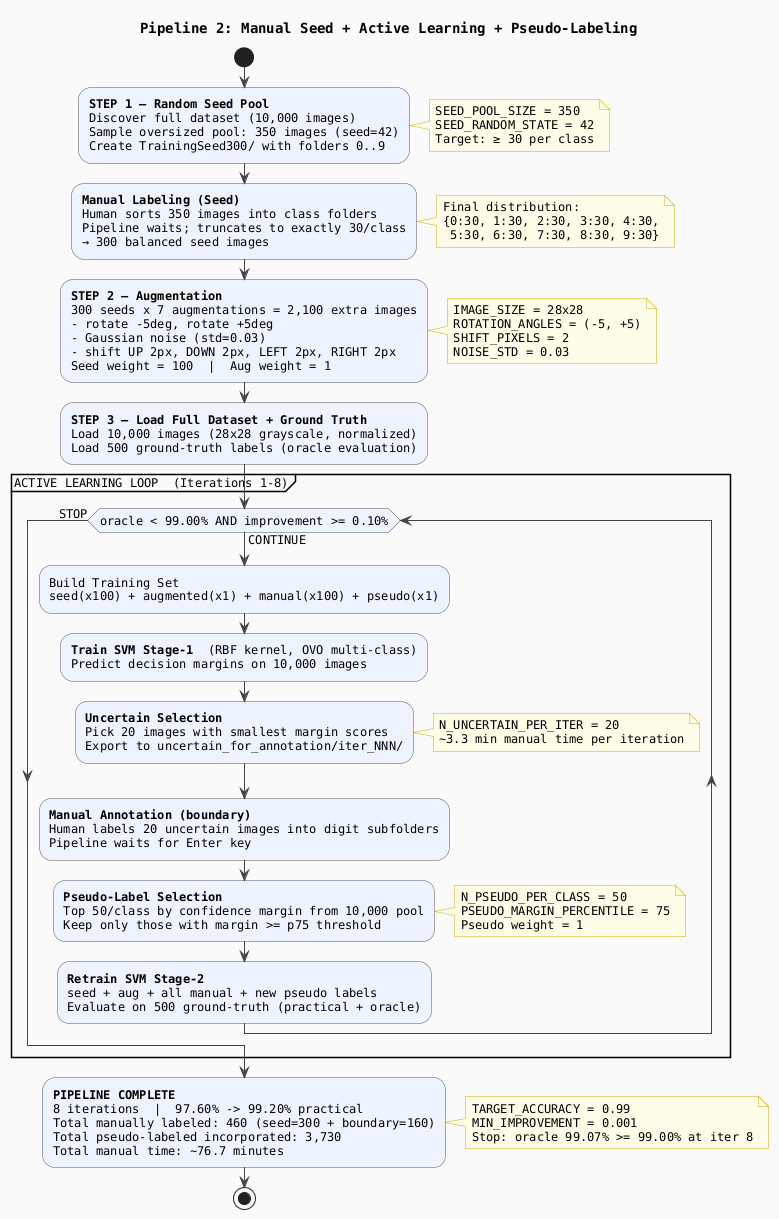
\includegraphics[width=0.6\textwidth]{figures/pipeline2/block diagram.png}
    \caption{Flow chart for pipeline 2 with the exact steps and values}
    \label{fig:pipeline2_block}
\end{figure}
\textbf{Pipeline Workflow}\\
The script follows this iterative lifecycle:
\begin{enumerate}
    \item Load and validate seed data.
    \item Augment seed images (7 synthetic samples per seed image).
    \item Train stage-1 SVM.
    \item Predict on full dataset.
    \item Export 20 most uncertain images for manual labeling.
    \item Wait for manual labels to be completed.
    \item Select high-confidence pseudo-labels from current predictions.
    \item Retrain stage-2 SVM with new manual + pseudo-labeled samples.
    \item Evaluate and check stopping criteria.
    \item If stopping criteria not met, return to step 4 with the retrained model.
\end{enumerate}
\textbf{Stopping Criteria}\\
The loop stops when one of the following is true:
\begin{itemize}
    \item Accuracy is at least 99%.
    \item Iteration-to-iteration improvement is below 0.1%.
\end{itemize}
If oracle evaluation is available, stopping uses oracle accuracy; otherwise practical accuracy is used.

\subsubsection{Simulation results}

\paragraph{Run setup and seed construction.}
The finalized run used all \textbf{10,000} images in \texttt{Indian\_Digits\_Train}. A random oversized pool of 350 images was first sampled for manual organization into class folders, then truncated to a balanced seed set of \textbf{300 images} (30 per class).
Each seed image produced \textbf{7} augmentations (2 rotations, 1 noise variant, and 4 directional shifts), giving \textbf{2100} augmented samples. A fixed practical subset of 500 labeled images was used for in-loop monitoring, and oracle scoring was computed with \texttt{check\_accuracy.p} after each iteration.

\paragraph{Iteration metrics.}
\begin{table}[H]
\centering
\caption{Pipeline 2 iteration metrics (active learning + pseudo-labeling)}
\label{tab:part3_pipeline2_iterations}
\resizebox{\textwidth}{!}{
\begin{tabular}{ccccccc}
\toprule
\textbf{Iter.} & \textbf{Practical (\%)} & \textbf{Oracle (\%)} & \textbf{Manual +} & \textbf{Pseudo +} & \textbf{Rejected (top-50/class)} & \textbf{Threshold} \\
\midrule
1 & 97.60 & 97.64 & 20 & 462 & 38/500 & 0.9933 \\
2 & 98.00 & 97.74 & 20 & 461 & 39/500 & 0.9942 \\
3 & 97.60 & 98.33 & 20 & 454 & 46/500 & 0.9946 \\
4 & 98.20 & 98.51 & 20 & 466 & 34/500 & 0.9948 \\
5 & 98.40 & 98.73 & 20 & 483 & 17/500 & 0.9945 \\
6 & 98.80 & 98.87 & 20 & 473 & 27/500 & 0.9949 \\
7 & 99.00 & 98.97 & 20 & 451 & 49/500 & 0.9953 \\
8 & 99.20 & 99.07 & 20 & 480 & 20/500 & 0.9949 \\
\bottomrule
\end{tabular}
}
\end{table}

\paragraph{Stopping condition and final totals.}
Stopping occurred at iteration 8 when the oracle target was reached:
\[
99.07\% \ge 99.00\%.
\]

\begin{itemize}
    \item Final practical accuracy: \textbf{99.20\%} (496/500).
    \item Final oracle accuracy: \textbf{99.07\%} (9907/10000).
    \item Iterations performed: \textbf{8}.
    \item Total manually labeled images: \textbf{460} (= 300 seed + 160 uncertain samples).
    \item Total pseudo-labeled images incorporated: \textbf{3730}.
    \item Estimated manual time: \textbf{4600 s} ($\approx 76.7$ min), using 10 s per manual label.
\end{itemize}

The active-learning loop improved practical measured accuracy from 97.60\% to 99.20\% and reached the assignment target on oracle evaluation.

\newpage
\subsection{Pipeline 3: Moondream Prototyping to Local CNN-Based Hybrid}

At the start of this track, we first experimented with vision-language models (mainly Moondream and LLaVA) to speed up labeling. In practice, API-key based inference had provider limits, quota/rate constraints, and unstable throughput. For a dataset size of 10,000 images, relying on external API calls was difficult to scale reliably.

Therefore, we moved to a local reproducible pipeline. The finalized method in this section is a \textbf{CNN-based hybrid transfer/fine-tuning workflow} (CNN backbone with practical preprocessing and shape-prior adaptation), rather than a purely standalone end-to-end CNN-only setup.

\subsubsection{Pipeline 3 Stages (Final Local Workflow)}

\begin{enumerate}
    \item \textbf{Initial staged training of the local CNN-based hybrid model on \texttt{AHDBase\_TrainingSet}.}
    The script \path{train_digits_staged.py} produced \path{runs/digits_staged}. The summary file reports best validation accuracy of \textbf{0.98125}.

    \item \textbf{Transfer evaluation on \texttt{PracticalGroundTruth500}.}
    The script \path{predict_digits_cnn.py} was used to compare transfer checkpoints; \path{stage_05.pt} transferred better than \path{best_model.pt} (43.00\% vs 41.20\%).

    \item \textbf{Support/query prototype adaptation on practical subset.}
    Using 3 support images per class (seed 7), autocontrast, and shape prior, the measured query accuracy reached \textbf{413/470 = 87.87\%}.

    \item \textbf{Fine-tuning on \texttt{PracticalGroundTruth500}.}
    Starting from \path{runs/digits_staged/stage_05.pt}, fine-tuning produced \path{runs/practical500_finetune/best_model.pt} with:
    \begin{itemize}
        \item best validation accuracy = \textbf{0.94}
        \item held-out test accuracy = \textbf{0.84}
    \end{itemize}

    \item \textbf{Full prediction on \texttt{Indian\_Digits\_Train}.}
    The final full run used \path{runs/practical500_finetune/best_model.pt} and produced predictions for all \textbf{10,000} images with no empty \texttt{predicted\_label} values.

    \item \textbf{Submission ordering correction.}
    Final predictions were sorted by numeric image ID (1,2,3,...) to avoid lexicographic-order mismatch during oracle-style evaluation.
\end{enumerate}

\subsubsection{Key Commands Used}

\noindent\textbf{Fine-tuning stage command.}
\begin{lstlisting}[language=bash]
python .\train_digits_staged.py \
    --data-dir .\PracticalGroundTruth500 \
    --resume-from .\runs\digits_staged\stage_05.pt \
    --stage-sizes 5,10,20,30,40 \
    --epochs-per-stage 20 \
    --patience 5 \
    --lr 1e-4 \
    --val-ratio 0.10 \
    --test-ratio 0.10 \
    --output-dir .\runs\practical500_finetune
\end{lstlisting}

\noindent\textbf{Final full prediction command.}
\begin{lstlisting}[language=bash]
python .\predict_digits_cnn.py \
    --checkpoint .\runs\practical500_finetune\best_model.pt \
    --input-dir .\Indian_Digits_Train \
    --support-dir .\PracticalGroundTruth500 \
    --autocontrast \
    --use-shape-prior \
    --shape-prior-weight 0.3 \
    --output-csv .\runs\indian_digits_cnn_finetuned_predictions.csv
\end{lstlisting}

\subsubsection{MATLAB Online Oracle Scoring (\texttt{check\_accuracy.p})}

For final local-model validation, we used MATLAB Online and the provided P-coded oracle file \path{check_accuracy.p}. The scoring input was a CSV prediction file containing labels for all 10,000 images.

\paragraph{MATLAB checker used for \texttt{predictions\_final.csv}.}
\begin{lstlisting}[language=Matlab]
% reduced MATLAB Online checker for predictions_final.csv
pred_file = 'predictions_final.csv';
T = readtable(pred_file);
fprintf('Scoring %s\n', pred_file);

assert(ismember('predicted_label', T.Properties.VariableNames), ...
    'predicted_label column not found');

preds = str2double(string(T.predicted_label));  % handles numeric/text columns
assert(~any(isnan(preds)), ...
    'Found %d missing predicted_label entries.', sum(isnan(preds)));
assert(numel(preds) == 10000, ...
    'predicted vector must have length 10000');

% Align to oracle order (1..10000) before scoring.
n = numel(preds);
ord = (1:n)';

if ismember('image_id', T.Properties.VariableNames)
    ids = str2double(string(T.image_id));
    assert(~any(isnan(ids)), ...
        'Found %d invalid image_id entries.', sum(isnan(ids)));
    [ids_sorted, ord] = sort(ids(:));
    assert(isequal(ids_sorted, (1:n)'), ...
        'image_id must be exactly 1..%d with no duplicates/missing rows.', n);
    preds = preds(ord);
    fprintf('Aligned predictions using image_id.\n');
elseif ismember('path', T.Properties.VariableNames)
    p = string(T.path);
    ids = nan(n, 1);
    for i = 1:n
        tok = regexp(p(i), '(\\|/)(\d+)\.[^\\/]+$', 'tokens', 'once');
        if ~isempty(tok)
            ids(i) = str2double(tok{2});
        end
    end
    assert(~any(isnan(ids)), ...
        ['Could not parse numeric image id from %d path entries. ' ...
         'Expected .../<number>.ext'], sum(isnan(ids)));
    [ids_sorted, ord] = sort(ids(:));
    assert(isequal(ids_sorted, (1:n)'), ...
        'Parsed path IDs must be exactly 1..%d with no duplicates/missing rows.', n);
    preds = preds(ord);
    fprintf('Aligned predictions using numeric ID parsed from path.\n');
else
    fprintf(['No image_id/path column found; using row order as-is. ' ...
             'Ensure rows already match oracle order.\n']);
end

preds_int = int32(preds(:));
try
    [acc, n_correct, n_total] = check_accuracy(preds_int);
    fprintf('accuracy=%.6f\ncorrect=%d/%d\n', acc, n_correct, n_total);
catch
    acc = check_accuracy(preds_int);
    fprintf('accuracy=%g\n', acc);
end
\end{lstlisting}

\paragraph{Output snippet (MATLAB Online).}
\begin{lstlisting}[language=Matlab]
>> check
Scoring predictions_final.csv
Aligned predictions using numeric ID parsed from path.

===== Classification Results =====
  Correct : 9339 / 10000
  Accuracy: 93.39%
==================================
\end{lstlisting}

\paragraph{Consistency note across Part 3 pipelines.}
The 93.39\% value above is the oracle score for the specific file \texttt{predictions\_final.csv} in this CNN run. It is reported independently from Pipeline 1 (99.09\%) and Pipeline 2 (99.07\%) results, since each pipeline uses different training/adaptation procedures and run configurations.

\subsubsection{Final Artifacts and Results}

\begin{table}[H]
\centering
\caption{Pipeline 3 final artifacts and measured outcomes}
\label{tab:part3_pipeline3_summary}
\begin{tabular}{>{\raggedright\arraybackslash}p{0.46\textwidth}>{\raggedright\arraybackslash}p{0.46\textwidth}}
\toprule
\textbf{Item} & \textbf{Value} \\
\midrule
Final checkpoint & \path{runs/practical500_finetune/best_model.pt} \\
Full prediction file & \path{runs/indian_digits_cnn_finetuned_predictions.csv} \\
Numeric-sorted prediction file & \path{runs/indian_digits_cnn_finetuned_predictions_numeric.csv} \\
Recommended submission file & \path{runs/indian_digits_cnn_finetuned_submission.csv} \\
Labels-only alternative & \path{runs/indian_digits_cnn_finetuned_labels_only.txt} \\
Practical subset match check (diagnostic) & 470/500 = 94.0\% \\
Oracle score for shown \texttt{predictions\_final.csv} & 9339/10000 = 93.39\% \\
Predictions generated in final run & 10,000 / 10,000 \\
\bottomrule
\end{tabular}
\end{table}

\paragraph{Manual effort note.}
For the 10,000-image final inference stage, no additional per-image manual labeling was needed; the pipeline relied on the already available labeled practical subset (\path{PracticalGroundTruth500}) plus local model inference.

\subsubsection{Additional Pipeline 3 Baseline: Qwen2-VL (Practical 500 Set)}

After finalizing the local CNN-based hybrid track, we also evaluated a separate Qwen2-VL baseline as an additional reference experiment. This Qwen run focused on the practical set workflow (500 labeled samples for evaluation) and was used to measure how far prompt/inference-only tuning can go without task-specific model fine-tuning.

\paragraph{Qwen baseline setup.}
\begin{itemize}
    \item Task: classify handwritten Arabic-Indic digits (0--9).
    \item Evaluation set: \path{Qwen/PracticalGroundTruth500} (500 labeled samples, class-balanced with 50 samples per class).
    \item Main workflow notebooks: \path{Qwen/scripts/create_labels_and_predection.ipynb}, \path{Qwen/scripts/resize_images.ipynb}, and \path{Qwen/scripts/compute_accuracy.ipynb}.
    \item Key hardening steps: robust output parsing, stable ground-truth merge, preprocessing with aspect-ratio-preserving resize/padding, and GPU-enabled execution path.
\end{itemize}

\paragraph{Qwen results summary.}
\begin{table}[H]
\centering
\caption{Pipeline 3 Qwen2-VL practical-set results}
\label{tab:part3_qwen_summary}
\begin{tabular}{>{\raggedright\arraybackslash}p{0.48\textwidth}>{\raggedright\arraybackslash}p{0.44\textwidth}}
\toprule
\textbf{Item} & \textbf{Value} \\
\midrule
Final practical accuracy & 112/500 = \textbf{22.40\%} \\
Invalid predictions in final run & \textbf{0} \\
Early failed state & 0/500 = 0.0\% (dominated by invalid parsing) \\
Intermediate stable checkpoints & 73/500 = 14.6\%, then 111/500 = 22.2\% \\
Prediction distribution note (final) & Strong class bias remained (e.g., class 2 over-predicted) \\
\bottomrule
\end{tabular}
\end{table}

\paragraph{Assignment reporting note.}
This Qwen2-VL result is reported as an additional practical-set baseline inside Pipeline 3. Since this run was evaluated on the practical 500-sample set (not full oracle scoring on 10,000 predictions), it is used for methodology comparison and debugging evidence, while the official Pipeline 3 full-dataset oracle figure remains the local-model result (93.39\%).

\subsection{Part 3 Cross-Pipeline Comparison}

Table~\ref{tab:part3_cross_pipeline} consolidates the finalized outcomes, including supplementary add-on baselines, so all reported Part 3 results can be compared directly.

\begin{table}[H]
\centering
\caption{Part 3 cross-pipeline comparison}
\label{tab:part3_cross_pipeline}
\begin{tabular}{>{\raggedright\arraybackslash}p{0.26\textwidth}>{\raggedright\arraybackslash}p{0.14\textwidth}>{\raggedright\arraybackslash}p{0.10\textwidth}>{\raggedright\arraybackslash}p{0.20\textwidth}>{\raggedright\arraybackslash}p{0.24\textwidth}}
\toprule
\textbf{Pipeline} & \textbf{Oracle Accuracy} & \textbf{Iterations} & \textbf{Manual Effort} & \textbf{Observation} \\
\midrule
Pipeline 1 (K-means bootstrapping + HITL SVM) & 99.09\% & 3 & 424 handled images, 1240.0 s & Highest oracle accuracy with the lowest estimated manual time among the two HITL-SVM pipelines. \\ \\
Pipeline 2 (active learning + pseudo-labeling SVM) & 99.07\% & 8 & 460 labels, 4600 s & Reached the 99\% target with stable gains, but required more manual actions and time than Pipeline 1. \\ \\
Pipeline 3 (Moondream prototyping -> local CNN-based hybrid) & 93.39\% & N/A & No additional per-image labels during final inference; reused \path{PracticalGroundTruth500} & Started from VLM prototyping, then shifted to a local CNN-based hybrid baseline; lower oracle accuracy under this run setup. \\ \\
Pipeline 3 add-on (Qwen2-VL prompt/inference baseline) & N/A (practical: 22.40\%) & N/A & No new labels; evaluated using existing 500 practical labels & Stable end-to-end after debugging (invalid=0), but strong class-bias limited final practical accuracy. \\ \\
\bottomrule
\end{tabular}
\end{table}

\paragraph{Comparative interpretation.}
\begin{itemize}
    \item Pipeline 1 and Pipeline 2 are nearly tied in oracle accuracy (difference = 0.02 percentage points).
    \item Pipeline 1 achieved this with less estimated manual effort than Pipeline 2 in the reported runs.
    \item Pipeline 3's local CNN-based hybrid run (93.39\% oracle) substantially outperformed the Qwen practical-set baseline (22.40\% practical).
    \item The Qwen baseline demonstrates a working VLM path, but practical-only scoring and class-bias behavior make it a supplementary reference, not the primary Pipeline 3 result.
\end{itemize}
\newpage
\subsection{Conclusion}
In Part 3, Pipeline 1 reached 99.09\% (9909/10000), Pipeline 2 reached 99.07\% (9907/10000), and the primary Pipeline 3 local-model run reached 93.39\% (9339/10000) for \texttt{predictions\_final.csv}. An additional Qwen2-VL baseline was also documented inside Pipeline 3, reaching 22.40\% on the practical 500-sample evaluation after full debugging and stabilization. Overall, the two human-in-the-loop SVM pipelines achieved the strongest performance, while Pipeline 3 now reports both a stronger local hybrid result and a practical-only VLM baseline for transparent comparison.